% Upload the complete ZIP to Overleaf; set this file as the main document.
% Compile with pdfLaTeX + BibTeX, or XeLaTeX + BibTeX.
% Author-review research draft. No results or author declarations are invented.
\documentclass[preprint,12pt,authoryear]{elsarticle}
\usepackage[T1]{fontenc}
\usepackage[utf8]{inputenc}
\usepackage{lmodern,amsmath,amssymb,booktabs,longtable,tabularx,graphicx}
\usepackage{microtype}
\usepackage{float}
\usepackage[margin=1in]{geometry}
\setlength{\emergencystretch}{2em}
\makeatletter
\def\inputrows#1{\@@input #1 }
\patchcmd{\ps@pprintTitle}{Preprint submitted to}{Research draft for}{}{}
\makeatother
\usepackage{xurl}
\usepackage[hidelinks]{hyperref}
\journal{The Journal of Finance and Data Science}
% Generated by scripts/build_jfds_research.py; do not hand-edit.
\newcommand{\FeatureCount}{30}
\newcommand{\PredictionCount}{5562}
\newcommand{\PanelDays}{2083}
\newcommand{\LogisticAccuracy}{52.95}
\newcommand{\InverseAccuracy}{52.88}
\newcommand{\PooledDifference}{0.07}
\newcommand{\PooledLow}{-1.44}
\newcommand{\PooledHigh}{1.61}
\newcommand{\GrossSharpe}{0.544}
\newcommand{\NetSharpe}{0.113}
\newcommand{\GrossLow}{-0.19}
\newcommand{\GrossHigh}{1.32}
\newcommand{\NetLow}{-0.60}
\newcommand{\NetHigh}{0.87}
\newcommand{\CostRoot}{11.36}
\newcommand{\RootLow}{-4.00}
\newcommand{\RootHigh}{26.43}
\newcommand{\Turnover}{0.766}
\newcommand{\DailyCost}{6.89}
\newcommand{\NetAnnualMean}{6.60}
\newcommand{\NetAnnualVol}{58.38}
\newcommand{\ExecutionSharpe}{-0.583}
\newcommand{\ExecutionReturn}{-94.61}
\newcommand{\EconomicDifference}{41.17}
\newcommand{\EconomicLow}{-4.89}
\newcommand{\EconomicHigh}{86.14}

\newcommand{\E}{\mathbb{E}}
\newcommand{\ind}{\mathbf{1}}
\newcommand{\draftnote}[1]{\par\noindent\textit{Author completion required: #1}\par}
\begin{document}
\begin{frontmatter}
\title{Beyond Directional Accuracy: A Reproducible Audit of Daily Cryptocurrency Forecasts and Trading Costs}
% Author identities belong in title_page.tex, not in the review manuscript.
\begin{abstract}
Directional forecasting accuracy, incremental predictive value, and trading profitability are different research outcomes. This study examines these distinctions through a reproducible audit of a cryptocurrency forecasting implementation. Using daily Binance spot data for Bitcoin, Ether, and Dogecoin, we construct \FeatureCount{} causal price, volume, trading-activity, and calendar features and evaluate logistic regression and histogram gradient boosting in expanding-window tests. The evaluation yields \PredictionCount{} out-of-sample asset-day predictions over \PanelDays{} distinct decision dates. Logistic regression achieves \LogisticAccuracy\% pooled accuracy, compared with \InverseAccuracy\% for a parameter-free inverse-persistence rule. A date-synchronized stationary bootstrap estimates an accuracy difference of \PooledDifference{} percentage points, with a 95\% interval of [\PooledLow, \PooledHigh]. An idealized equal-weight long/short return diagnostic has gross annualized Sharpe \GrossSharpe{} and net Sharpe \NetSharpe{} at an assumed nine basis points per unit of one-way turnover. Joint resampling of gross returns and turnover gives a break-even cost estimate of \CostRoot{} basis points, with a 95\% interval of [\RootLow, \RootHigh]. A separate next-open-to-close cash ledger illustrates the sensitivity to mandatory daily liquidation. Regression fixtures detect eight deliberately introduced software mutations. The results do not establish incremental superiority over the reversal baseline or robust trading profitability. The contribution is an auditable case study linking prediction, uncertainty, implementation contracts, and economic evaluation, rather than a claim of a new forecasting algorithm.
\end{abstract}
\begin{keyword}
Cryptocurrency \sep Directional forecasting \sep Walk-forward evaluation \sep Backtesting \sep Transaction costs \sep Reproducibility
\end{keyword}
\end{frontmatter}

\section{Introduction}
An accurate classifier need not be an economically useful trading system. A directional prediction receives the same credit for correctly forecasting a small move as a large one, whereas trading profits depend on signed return magnitudes, position sizes, implementation timing, and costs. A second distinction is equally important: a classifier can exceed a 50\% hit rate while offering little additional information relative to a simple observable rule. A third concerns measurement itself. A backtest may apply a model consistently yet implement the wrong execution or accounting convention.

This paper studies these issues in one supplied cryptocurrency forecasting artefact. The empirical question is narrow: do technical-feature classifiers improve next-day directional accuracy over elementary baselines on the same dates, and what economic conclusions remain under explicit cost and execution assumptions? The engineering question is whether executable tests detect selected faults that could compromise the interpretation of the result. These are separate questions; neither statistical significance nor passing software tests answers both.

The study makes three contributions. First, it provides a complete prediction-level replication with a reconciled sample, fold-specific preprocessing, saved fitted pipelines, and a feature inventory tied to executable code. Second, it measures model--baseline differences with serial-dependence-aware per-asset inference and synchronized date-block resampling, and estimates the cost root directly from jointly resampled returns and turnover. Third, it separates an idealized target-notional return diagnostic from a fully liquidated daily cash-ledger experiment, while documenting the scope of regression and mutation tests.

The main finding is not that cryptocurrency cannot be forecast. It is that the additional value of the tested classifiers over inverse persistence is not established in this sample. The pooled accuracy difference is small relative to its uncertainty. The financial result is also sensitive to costs and the trading policy translating forecasts into positions. These findings support a reproducibility and evaluation case study, not a universally profitable strategy or a claim about all cryptocurrency models.

\section{Related research and positioning}
Research on cryptocurrency predictability provides mixed findings across horizons, inputs, and model classes. \citet{jaquart2021}, in this journal, examine Bitcoin prediction horizons from one to sixty minutes and compare several machine-learning models. Their setting differs from this paper's daily, three-asset study. \citet{gradojevic2023} consider technical predictors at hourly and daily frequencies and report that forecasting results depend on horizon and specification. These studies motivate explicit statements of sampling frequency, benchmarks, and input information; they do not imply that their reported performance should transfer to the present data or implementation.

\citet{arnott2019} discuss disciplined financial backtesting in the machine-learning setting. Our contribution is an executable, single-artefact application of that general research concern. We do not introduce a new model family or establish the prevalence of software defects across published research. The provenance problem is related to the formulation of data leakage in \citet{kaufman2012}: information must be assessed relative to its availability for the prediction task, rather than inferred from a variable's name.

For inference, the paired forecast-comparison perspective of \citet{diebold1995} motivates analyzing observation-level loss differences. We use a Bartlett-kernel heteroskedasticity and autocorrelation consistent (HAC) estimate following \citet{newey1987}. The cross-asset analysis uses the stationary bootstrap of \citet{politis1994}, with a single resampled date index applied to all asset columns. Finally, mutation testing, reviewed by \citet{jia2011}, evaluates whether selected erroneous implementations are detected by tests. It provides conditional evidence about those mutations, not proof that the entire system is correct.

\section{Research artefact and data provenance}
\subsection{Scope of the implemented model}
The empirical implementation is a daily technical-feature forecasting pipeline with logistic and boosted-tree classifiers. An additional one-feature logistic model is a diagnostic ablation. The broader software repository contains components for other forecasting and text-processing workflows; those components are not trained or validated in this experiment. In particular, the reported results are not evidence for an LLM, FinBERT, Prophet, recurrent-network ensemble, live exchange service, or autonomous trading deployment.

The experiment is retrospective. The initial model settings are inherited from the supplied evaluation source; no new search for an attractive test-period configuration is performed. However, no preregistration or untouched final holdout is available, and the comparisons and audit checks were developed with knowledge of the existing artefact. Consequently, the results are replication and exploratory evidence, not prospective confirmation of a selected strategy.

\subsection{Market data and sample reconciliation}
The inputs are frozen daily Binance spot klines for BTCUSDT, ETHUSDT, and DOGEUSDT. The stored fields include open, high, low, close, base volume, quote volume, trade count, and taker-buy base volume. The exchange documents the kline format and public archive \citep{binance2026}. Bar dates refer to UTC opening dates; the entire day's bar is available only after that day ends.

BTC and ETH raw histories run from 17 August 2017 through 1 April 2026, while DOGE begins on 5 July 2019. The validation checks find no duplicate or missing daily dates in these files, and enforce positive prices and consistent OHLC bounds. SHA-256 hashes identify the exact supplied inputs. An additional read-only check compares eight numeric fields for 275 overlapping asset-days in July 2019, January 2023, and March 2026 with the exchange's checksum-verified monthly archives. All compared fields match within relative tolerance $10^{-10}$ and absolute tolerance $10^{-8}$. This is a selected-month verification, not an independent audit of every historical observation.

\begin{table}[htbp]
\centering\small
\caption{Sample reconciliation. Every asset has a final decision date of 30 March 2026. The final realized label date is 31 March 2026.}\label{tab:sample}
\begin{tabular}{lrrrrl}\toprule
Asset & Raw rows & Usable & OOS & Folds & First OOS decision\\\midrule
\inputrows{generated/sample.tex}
\bottomrule\end{tabular}
\end{table}

Feature warm-up removes the first 60 rows. The final two raw bars are excluded as prediction origins to preserve the supplied study's cutoff: one supports the final included label, and the last is an unused buffer. This explains why the usable count is raw rows minus 62, although the classification horizon itself is only one day. Initial training and the five-row gap then account for 1,005 usable rows per asset before evaluation begins (Table~\ref{tab:sample}). There are \PredictionCount{} asset-day forecasts but only \PanelDays{} distinct decision dates. These counts must not be interchanged when discussing dependence or effective information.

\subsection{Why the sentiment proxy is excluded}
The supplied sentiment-generation script explicitly describes a simulation based on a market proxy. It constructs an intraday return $u_t=(C_t-O_t)/O_t$, then a score
\begin{equation}
 s_t=\operatorname{round}_3\!\left[\operatorname{clip}\!\left(
 \operatorname{clip}(15u_t,-1,1)+\epsilon_t,-1,1\right)\right],
 \qquad \epsilon_t\sim U(-0.2,0.2).
\end{equation}
Its associated headline is selected from fixed templates according to the score. This is not an independent historical news source, and the original generator does not fix the random seed. It is therefore excluded from all model inputs and results in this paper.

Using this score to predict the same bar before the bar closes would violate the information boundary. Using it after the close to predict a later return is not automatically look-ahead leakage; it is a noisy transformation of already-observed price information. A high contemporaneous correlation alone cannot determine which problem applies. The appropriate audit records construction, source, availability time, and target alignment. We do not infer misconduct from a generator that already labels itself a simulation, or make claims about genuine text-based sentiment models.

\section{Methods}
\subsection{Features, target, and information boundary}
Let $\mathcal F_t$ contain complete market bars through the close of day $t$. Each feature vector $x_t$ is a function of $\mathcal F_t$. The binary target and associated simple return are
\begin{equation}
 y_t=\ind(C_{t+1}>C_t),\qquad r_{t+1}=C_{t+1}/C_t-1.
\end{equation}
A tie belongs to class zero. Binary labels do not imply a 50\% unconditional up probability; therefore, a coin flip is not the only relevant benchmark. The executable feature matrix contains \FeatureCount{} columns, not the 34 stated in the supplied draft. \ref{app:features} gives all definitions. No full-sample imputation, cross-asset predictors, sentiment proxy, or forward-return variable enters training.

\subsection{Expanding-window evaluation and model fitting}
For each asset, index usable observations by $i=0,\ldots,n-1$. Fold starts are $a_k=1005+250k$. Training uses $i<a_k-5$, and testing uses $a_k\leq i<\min(a_k+250,n)$. A final test block is retained only if it contains at least 30 observations. The earliest fold has 1,000 training rows; later training sets expand. Every reported observation is predicted exactly once out of sample.

A standard scaler is fitted separately on each training fold and remains unchanged during that fold's prediction. Both the fitted scaler and classifier are saved together. The implementation exports the last training-feature date, last training-label date, and test dates, so the information gap can be checked directly. Five excluded rows provide separation for the one-day labels. This is not a claim that all historical feature windows are disjoint: shared past observations in causal rolling features do not by themselves constitute future-information leakage.

The logistic model uses $\ell_2$ regularization with inverse penalty parameter $C=0.1$, an intercept, and a maximum of 2,000 iterations. Histogram gradient boosting uses maximum depth three, 200 boosting iterations, learning rate 0.05, $\ell_2$ leaf regularization one, no early stopping, and random seed zero. These settings are fixed across assets and folds. Predictions use probability greater than 0.5 for class one, with ties assigned to zero. A lag-1-only logistic model uses the same penalty and fitting protocol, but retains only $\log(C_t/C_{t-1})$. It is reported as an ablation rather than selected as the preferred strategy.

\subsection{Baselines and estimands}
Persistence predicts yesterday's realized close-to-close direction, $\widehat y_t^{P}=\ind(C_t>C_{t-1})$. Inverse persistence predicts $1-\widehat y_t^P$. Both require no fitted parameter and are evaluated on exactly the model's dates. The majority baseline predicts the more frequent class in the current training fold, with ties assigned to zero. A long-only basket is a separate return benchmark, not a directional classifier.

For a model $M$ and inverse-persistence baseline $I$, the primary per-observation comparison is
\begin{equation}
 d_{j,t}=\ind(\widehat y^M_{j,t}=y_{j,t})-
          \ind(\widehat y^I_{j,t}=y_{j,t}).
\end{equation}
We report each asset's mean difference and confidence interval. A positive difference favors the model. We also report pooled accuracy as the descriptive fraction of correctly classified asset-days. Its paired difference is observation-weighted, $\widehat\Delta=\sum_{j,t}d_{j,t}/N$, rather than an equal-weight average of three asset accuracies.

\subsection{Dependence-aware uncertainty}
For a single asset, let $n$ be its OOS count and $v_t=d_t-\bar d$. The HAC variance of the mean is
\begin{equation}
 \widehat{\operatorname{Var}}(\bar d)=\frac1n\left[
 \widehat\gamma_0+2\sum_{\ell=1}^{K}\left(1-\frac{\ell}{K+1}\right)\widehat\gamma_\ell\right],
 \quad \widehat\gamma_\ell=\frac1n\sum_{t=\ell+1}^{n}v_tv_{t-\ell},\quad K=20.
\end{equation}
Intervals use the normal approximation and two-sided $p$-values. These are approximate dependent-data comparisons, not exact small-sample tests. The zero-variance, nonzero-difference case is explicitly marked undefined rather than assigned a nonsignificant $p$-value.

For pooled inference and return statistics, we use 2,000 circular stationary-bootstrap replicates with mean block length 20 dates and fixed seed 20260401. At each step, an index continues to the next observed date with probability $1-1/L$, or restarts at a uniformly sampled date with probability $1/L$. The same sampled date is applied to all assets, including the missing-asset mask. The pooled numerator and denominator are recomputed in every replicate. This preserves contemporaneous dependence within the resampled panel; pooling asset-days as independent Bernoulli trials would not.

We report percentile 95\% intervals and repeat the bootstrap with mean lengths five and 60. Forecasts are not refitted within each replicate, so inference is conditional on the fitted walk-forward predictions. Dependence adjustments do not eliminate structural breaks or uncertainty from prior researcher choices. All secondary model and policy comparisons are exploratory. We do not make multiplicity-adjusted discovery claims or interpret a failure to reject as proof of equivalence.

\subsection{Target-notional return and cost diagnostic}
On date $t$, let $A_t$ be the assets with OOS forecasts and let $J_t=|A_t|$. For each active asset, set $s_{j,t}=2\widehat y_{j,t}-1$ and target signed weight $w_{j,t}=s_{j,t}/J_t$. Other weights are zero. Gross diagnostic return and one-way target turnover are
\begin{equation}
 g_{t+1}=\sum_j w_{j,t}r_{j,t+1},\qquad
 q_t=\sum_j|w_{j,t}-w_{j,t-1}|,\qquad
 n_{t+1}(c)=g_{t+1}-c q_t.
\end{equation}
The initial target is zero. Final liquidation adds $\sum_j|w_{j,T}|$ to the final turnover observation. A complete sign reversal costs two units of notional. The reference cost is $c=0.0009$, interpreted as four basis points of fees plus five of slippage per unit of one-way turnover. These are scenario assumptions, not verified exchange fee schedules or calibrated market-impact estimates.

This is a linear target-notional diagnostic. Turnover ignores position-weight drift and cost-induced changes in sizing; it is not an exact self-financing account. Its close-to-close return window also assumes the day's closing information is actionable at the boundary without additional latency. The diagnostic is useful for separating signed-return forecasts from turnover costs, but it must not be relabeled as realized execution performance. The portfolio has unit gross exposure when all signals are active; it is directional and need not be market neutral.

Annualized Sharpe is $S=\sqrt{365}\,\bar n/s_n$, with sample standard deviation and zero risk-free rate. We report annualized arithmetic mean $365\bar n$ and volatility $\sqrt{365}s_n$ separately. The exact zero-mean cost root within this linear diagnostic is
\begin{equation}\label{eq:root}
 c^*_{\mathrm{bps}}=10^4\frac{\bar g}{\bar q},\qquad \bar q>0.
\end{equation}
Each bootstrap replicate jointly resamples $(g_t,q_t)$ and recomputes this ratio and net Sharpe. We do not infer the root by interpolating Sharpe or hold turnover fixed when estimating its interval. A negative root means that the resampled gross mean is already negative at zero cost; it is not a feasible negative transaction charge and is not clipped to zero.

\subsection{A distinct fixed-horizon execution experiment}
To examine an explicit bar-level trading policy, a second calculation enters at $O_{t+1}$ and exits at $C_{t+1}$ every day, including when the following signal has the same direction. It therefore closes and reopens exposure instead of netting repeated target weights. Each asset receives $1/J_t$ of equity measured before any same-day entry. No same-day closing price is used to size another asset's trade.

For side $s\in\{-1,+1\}$, adverse slippage $\lambda=0.0005$, and fee rate $f=0.0004$, define
\begin{equation}
 P_{\mathrm{in}}=O_{t+1}(1+s\lambda),\quad
 P_{\mathrm{out}}=C_{t+1}(1-s\lambda),\quad
 R=s\left(\frac{P_{\mathrm{out}}}{P_{\mathrm{in}}}-1\right)
      -f\left(1+\frac{P_{\mathrm{out}}}{P_{\mathrm{in}}}\right).
\end{equation}
The cash ledger independently books signed entry and exit notionals and each leg's own fee, then checks agreement with this formula. Positions are flat at each daily end. Starting equity is 10,000 accounting units, initial capital is included when calculating the first return, and Sharpe uses only the OOS earning window. There are no entry-bar stop/target assumptions, overlapping two-day returns, or unused pre-evaluation years in this calculation. Instantaneous access to the next bar open remains an idealization: daily data do not identify inference latency, queue priority, or market impact.

\section{Results}
\subsection{Directional accuracy and incremental value}
Table~\ref{tab:accuracy} reports all classifiers and elementary baselines. Logistic accuracy is \LogisticAccuracy\%, while inverse persistence attains \InverseAccuracy\%. The lag-1 ablation and boosted trees do not establish an improvement over the parameter-free baseline. Similar aggregate accuracies alone would not establish similar information content, since models may disagree on individual observations; the paired results supply the relevant comparison.

\begin{table}[htbp]\centering\small
\caption{OOS accuracy (percent). Pooled values are descriptive asset-day averages, not independent-observation significance tests.}\label{tab:accuracy}
\begin{tabular}{lrrrr}\toprule
Predictor & BTC & ETH & DOGE & Pooled\\\midrule
\inputrows{generated/accuracy.tex}
\bottomrule\end{tabular}\end{table}

\begin{table}[htbp]\centering\small
\caption{Paired accuracy differences relative to inverse persistence. Differences and confidence limits are in percentage points; HAC uses 20 lags. The additional model comparisons are exploratory.}\label{tab:paired}
\begin{tabular}{llrrr}\toprule
Asset & Model & Difference & 95\% interval & Two-sided $p$\\\midrule
\inputrows{generated/paired.tex}
\bottomrule\end{tabular}\end{table}

Per-asset logistic differences are approximately $-0.29$, $+0.53$, and $-0.07$ percentage points for BTC, ETH, and DOGE, respectively (Table~\ref{tab:paired}). Every interval crosses zero. The synchronized date bootstrap gives a pooled difference of \PooledDifference{} percentage points, with a 95\% interval [\PooledLow, \PooledHigh]. These estimates do not demonstrate incremental superiority. They also do not exclude modest gains or losses; there is no prespecified equivalence margin.

\begin{figure}[htbp]\centering
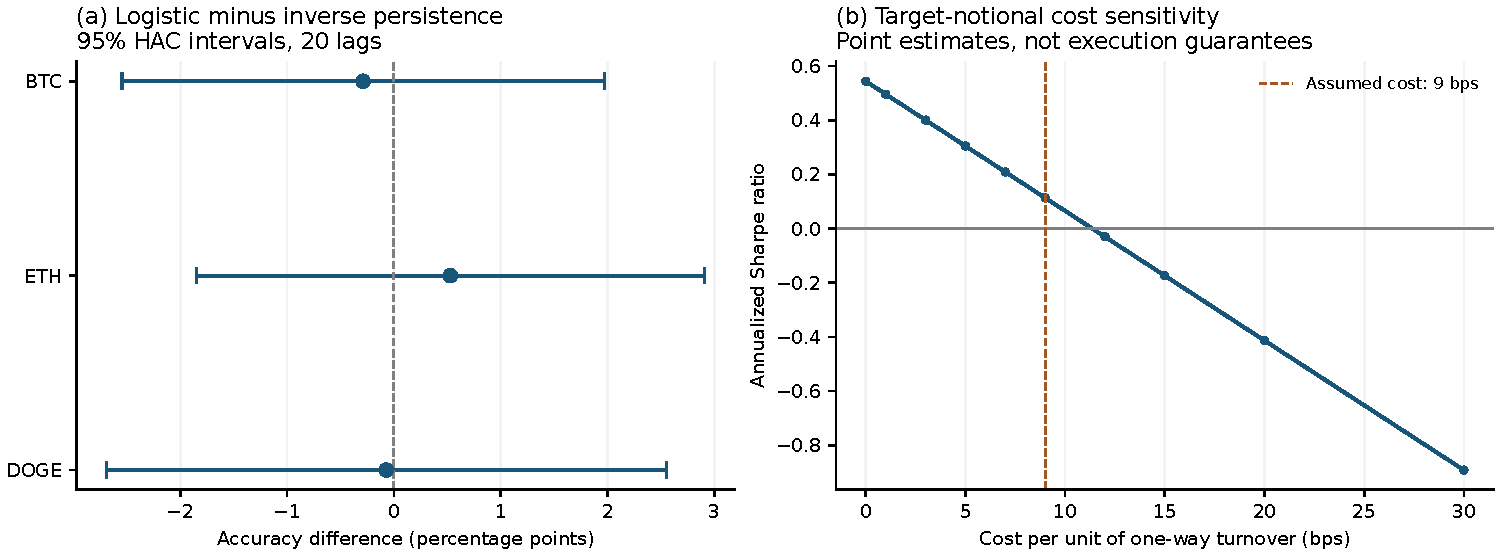
\includegraphics[width=\textwidth]{figures/evidence.pdf}
\caption{Two distinct evaluation questions. Panel (a) shows paired predictive differences with dependence-aware intervals. Panel (b) shows point-estimate economic sensitivity for the target-notional diagnostic; the curve is not a confidence band or a live execution forecast.}\label{fig:evidence}
\end{figure}

\ref{app:folds} reports every fold's dates, size, and model and baseline accuracy. The final folds have lower accuracy than several earlier folds, but this descriptive pattern is not a formal structural-break finding. Fold sizes differ at the sample end, and averaging fold percentages without weighting would change the estimand.

\subsection{Costs and uncertainty}
The logistic target-notional diagnostic has gross Sharpe \GrossSharpe{}, with stationary-bootstrap interval [\GrossLow, \GrossHigh]. At nine basis points, net Sharpe is \NetSharpe{}, with interval [\NetLow, \NetHigh]. Mean target turnover is \Turnover{} per day, implying a cost deduction of \DailyCost{} basis points per day. Annualized net arithmetic mean and volatility are \NetAnnualMean\% and \NetAnnualVol\%, respectively. The annualized mean is not a compounded investment return.

The point-estimate cost root is \CostRoot{} basis points, but its 95\% interval spans [\RootLow, \RootHigh]. The negative lower bound is economically informative: some resampled paths have negative gross expected return before charging any cost. The width of the interval prevents a precise claim that a particular executable cost level lies safely below break-even. Conversely, an interval crossing zero does not prove that the true expected return is exactly zero.

\begin{table}[htbp]\centering\small
\caption{Sensitivity of 95\% bootstrap intervals to mean block length. Accuracy differences are percentage points; cost roots are basis points. All variants use 2,000 synchronized replicates.}\label{tab:bootstrap}
\begin{tabular}{rrrrr}\toprule
Block length & Pooled difference & Gross Sharpe & Net Sharpe & Cost root\\\midrule
\inputrows{generated/bootstrap.tex}
\bottomrule\end{tabular}\end{table}

Table~\ref{tab:bootstrap} makes the dependence specification visible. These alternatives test sensitivity to the resampling scale, not robustness to every possible form of nonstationarity. The complete deterministic cost curve and gating variants are reported in \ref{app:sensitivity} rather than used to select a favorable threshold.

\subsection{Policy and benchmark sensitivity}
Table~\ref{tab:variants} gives target-notional return results for all prediction rules, a common three-asset window, and a logistic long/cash variant. The common-window analysis removes the changing asset count from the primary panel, while the long/cash version avoids the assumption of unrestricted short exposure. Neither is treated as a newly selected best policy. All net values in this table still use the approximate target-turnover convention.

\begin{table}[htbp]\centering\small
\caption{Exploratory target-notional policy comparisons at nine basis points. The common-window calculation starts the portfolio from cash on its own first date.}\label{tab:variants}
\begin{tabular}{lrrrr}\toprule
Variant & Days & Gross SR & Net SR & Turnover\\\midrule
\inputrows{generated/variants.tex}
\bottomrule\end{tabular}\end{table}

Similar hit rates do not imply identical return performance. For example, inverse persistence has gross Sharpe about 0.004 in this diagnostic, compared with \GrossSharpe{} for logistic regression. Joint date-block resampling gives an annualized arithmetic net-mean advantage for logistic over inverse persistence of \EconomicDifference{} percentage points, with a 95\% interval [\EconomicLow, \EconomicHigh]. This exploratory economic comparison is uncertain, but it shows why an inconclusive accuracy comparison cannot justify the stronger claim that the model adds no economically relevant information. The positive point estimates for the common-window and long/cash variants also preclude a blanket statement that every tested policy is unprofitable.

The passive reference uses the same available-asset set as the strategy on every date, with positive equal weights. Thus BTC and ETH each receive one half before DOGE becomes eligible, and all three receive one third thereafter. This is a gross rebalanced long-only basket, not a fixed-share buy-and-hold portfolio. Its correlation, beta, and untested intercept relative to the net strategy are exported for descriptive use. We do not infer an absence of alpha from an intercept point estimate or equate a lower raw Sharpe with an invalid diversification role.

The separate daily-liquidation execution experiment produces \PredictionCount{} round trips and \PanelDays{} daily equity returns. Under its stated sizing and cost policy, annualized Sharpe is \ExecutionSharpe{} and cumulative return is \ExecutionReturn\%. The magnitude of this loss is not a forecast of live trading performance; it is the outcome of an explicitly costly policy that repurchases or resells the full daily allocation even when signals persist. Daily cash reconciliation error is below $5\times10^{-12}$ accounting units, and final positions are flat. This calculation differs from the target-notional diagnostic in holding, cost realization, timing, and compounding. Their difference cannot be causally assigned to latency or any single software correction.

\section{Software verification and audit boundaries}
The regression suite for the existing backtest and feature-pipeline components contains 29 tests. It checks next-bar entry scheduling, asset-specific prices, short mark-to-market direction, stop-price behavior on tested bars, hold-expiry contracts, annualization from equity-curve cadence, resampling, cash reconciliation, scaler persistence, and chronological split contracts. The new research checks additionally test causal feature-prefix invariance, known-answer HAC variance, rejection of invalid statistics, joint resampling, benchmark weights, terminal target liquidation, the exact cost root, own-notional fees, saved-model predictions, and fold/result reconciliation.

Mutation testing changes one implementation behavior at a time and reruns the existing 29-test suite. A mutation is considered detected only if the expected named regression test fails, the total completed test count matches baseline, and the process exit status is consistent. Collection errors, missing tests, and skipped-test runs are not counted as successful detection. Table~\ref{tab:mutations} reports eight selected mutants, all detected.

\begin{table}[htbp]\centering\small
\caption{Selected software mutations. Counts refer to failed tests among the baseline 29. The eight mutants are deliberately chosen, not a random sample of possible defects.}\label{tab:mutations}
\begin{tabular}{lrl}\toprule
Introduced behavior & Failed tests & Outcome\\\midrule
\inputrows{generated/mutations.tex}
\bottomrule\end{tabular}\end{table}

This result does not imply complete branch coverage, that all historical faults were independently reproduced, or that eight tests establish economic validity. In particular, the split-gap mutation verifies a specified contract; it does not prove that every split without a five-row gap necessarily leaks information. Similarly, an execution fixture cannot determine whether an external feature was observable at a forecast timestamp.

The supplied draft also described randomized engine tests as a calibrated null experiment. We do not use that claim as empirical evidence here: its 2,400 fifteen-minute bars represent 25 days per path, not 75, and exponentiating zero-mean Gaussian increments gives zero log drift rather than zero expected simple return. A distributional diagnostic would additionally need consistent risk-free-rate treatment and terminal liquidation. Historical extreme Sharpe values and a twelve-fault narrative are therefore not used to make a quantitative causal attribution in this revision. The manuscript's verified engineering claims are restricted to the executable tests and selected mutations actually supplied and rerun.

\section{Discussion and limitations}
The central lesson concerns the estimand. Accuracy measures whether a direction is correct; paired accuracy measures whether a model adds to a baseline; a signed-return series measures magnitude-sensitive performance; a cash ledger measures the consequences of a particular trade policy. These objects can disagree without contradiction. Here, a seemingly attractive aggregate hit rate is closely matched by inverse persistence, and a positive gross Sharpe is accompanied by substantial uncertainty and cost sensitivity.

The study supports several practical reporting choices. Prediction records should carry decision dates, label dates, fold identifiers, probabilities, and baseline decisions. Preprocessing must be part of the saved model rather than an unspecified external step. Cost analysis should report the convention for one-way versus round-trip turnover and include initial and terminal actions. Finally, software tests should publish their exact scope and expected failure behavior. These recommendations follow from this artefact's measurement problems, not from a claim that the same problems affect every published study.

The limits are material. The evidence concerns three retrospectively chosen surviving assets at one exchange and a UTC daily boundary. It does not address delisted assets, selection bias across a broader universe, other exchanges, or re-anchored bars. Public archive spot checks increase confidence in selected inputs, but are not a full-history verification or proof against exchange revisions. The 30 features omit order books, funding, basis, open interest, liquidations, cross-asset information, and independently timestamped text.

The models are modest fixed specifications rather than an exhaustive comparison with modern architectures. Logistic probabilities are not externally calibrated. Optimizing classification loss does not optimize a turnover-aware investment objective. The OOS folds remain retrospective because the source analysis was inspected before this revision, and an untouched prospective validation period is still needed before any deployment claim.

HAC and the stationary bootstrap address selected dependence structures, not arbitrary regime shifts. The bootstrap does not refit the model or model estimation uncertainty under alternative research paths. Wide confidence intervals limit claims of both superiority and inferiority. Secondary models, gates, and portfolio variants are exploratory; no familywise discovery guarantee is provided.

Economically, spot prices do not make shorting automatically feasible. Borrowing constraints, margin requirements, liquidation, financing, funding, capacity, and size-dependent impact are absent. The long/cash diagnostic is a useful sensitivity but still not a live implementation. The target-notional approach omits weight drift, and the daily-liquidation ledger uses idealized bar-boundary fills. No measured exchange latency, paper trading, or broker/exchange reconciliation is available. None of the reported ratios should be interpreted as an expected investor return.

\section{Conclusion}
This reproducible audit evaluates a \FeatureCount{}-feature daily cryptocurrency forecasting implementation using explicit chronological folds, elementary baselines, dependent-data uncertainty, and auditable economic conventions. Logistic regression achieves \LogisticAccuracy\% accuracy over \PredictionCount{} OOS asset-days, compared with \InverseAccuracy\% for inverse persistence. The paired difference is small and uncertain, and the result does not establish incremental superiority. A gross Sharpe of \GrossSharpe{} falls to \NetSharpe{} under the reference target-turnover cost scenario, while a distinct daily-liquidation policy has materially different outcomes. Eight selected software mutations are detected, with the coverage boundary stated explicitly. The contribution is a transparent research artefact and a carefully bounded negative or inconclusive result, not a new universally superior forecasting model or a proven deployable strategy.

\section*{Data and code availability}
The local replication package contains the frozen input files, source code, fitted fold pipelines, dated predictions, trade ledger, machine-readable results, checksums, and reproduction instructions. The manuscript's numeric macros and tables are generated from these results. No public DOI or archival deposit has yet been assigned. Authors must confirm redistribution rights and arrange an anonymized reviewer supplement or an appropriate repository deposit before submission. No public release is implied by preparation of the local package.

\section*{Funding}
\draftnote{Confirm funding sources and funder roles, or supply an accurate no-funding statement.}
\section*{Declaration of competing interests}
\draftnote{All authors must confirm competing interests and complete the publisher's required declaration.}
\section*{Ethics and consent}
The reported empirical analysis uses market-price and trading-activity bars, not human-participant records or personal social-media data. No human-participant experiment is described. Authors should confirm any institutional requirements applicable to their work.
\section*{Declaration of generative AI and AI-assisted technologies in the writing process}
OpenAI Codex was used to assist with manuscript drafting and revision. AI assistance was also used to develop and check research code; this is disclosed separately from the writing use. \draftnote{The human authors must independently review the methods, code, numerical outputs, references, and wording; verify compliance with the journal's AI policy; and finalize a truthful disclosure and accountability statement. This draft does not assert that this review has already occurred.}

\appendix
\section{Complete feature definitions}\label{app:features}
Let $O,H,L,C,V,Q,N,B$ denote open, high, low, close, base volume, quote volume, trade count, and taker-buy base volume. Let $\mu_k$ and $\sigma_k$ be trailing $k$-bar mean and sample standard deviation ($\mathrm{ddof}=1$), and $z_k(X)=(X-\mu_k(X))/\sigma_k(X)$. Every rolling window ends at $t$. Undefined ratios become missing and are removed before fitting.
\begin{longtable}{p{0.21\textwidth}rp{0.63\textwidth}}
\caption{Executable feature inventory. Counts sum to 30.}\\\toprule
Group & Count & Definitions\\\midrule\endfirsthead
\toprule Group & Count & Definitions\\\midrule\endhead
Log returns & 6 & $\log(C_t/C_{t-k})$, $k\in\{1,2,3,5,10,20\}$.\\
Volatility/location & 8 & $\sigma_k(\log(C_t/C_{t-1}))$ and $z_k(C_t)$, $k\in\{5,10,20,60\}$.\\
Bar shape & 3 & $(H-L)/C$, $(C-O)/O$, $(C-L)/(H-L)$.\\
Trading activity & 7 & $B/V$, $\mu_5(B/V)$, $Q/N$, $z_{60}(Q/N)$, $z_{60}(N)$, $z_{60}(V)$, $V/\mu_{20}(V)$.\\
Technical/calendar & 6 & RSI, MACD histogram, Bollinger position, normalized ATR, sine and cosine of weekday, defined below.\\\bottomrule
\end{longtable}
With $\delta_t=C_t-C_{t-1}$, RSI is $100-100/[1+\mu_{14}(\max(\delta,0))/\mu_{14}(\max(-\delta,0))]$. This uses simple rolling averages, not Wilder's recursive smoothing. The MACD histogram is $M-\mathrm{EMA}_9(M)$, where $M=\mathrm{EMA}_{12}(C)-\mathrm{EMA}_{26}(C)$. Exponential means use $\alpha=2/(k+1)$, recursive initialization at the first observation, and \texttt{adjust=False}. Bollinger position is $(C-\mu_{20}(C))/(2\sigma_{20}(C))$. True range is $\max\{H-L,|H-C_{t-1}|,|L-C_{t-1}|\}$; normalized ATR is its simple 14-bar mean divided by $C$. Calendar features are $\sin(2\pi d/7)$ and $\cos(2\pi d/7)$ for weekday $d=0,\ldots,6$. The fields summarize daily exchange activity; they are not order-book snapshots.

\section{Complete fold results}\label{app:folds}
\begin{longtable}{lrlrrrr}
\caption{Fold-level OOS accuracy in percent; L denotes logistic and I inverse persistence. Dates are prediction origins.}\\\toprule
Asset & Fold & Start & End & $n$ & L & I\\\midrule\endfirsthead
\toprule Asset & Fold & Start & End & $n$ & L & I\\\midrule\endhead
\inputrows{generated/folds.tex}
\bottomrule\end{longtable}

\section{Additional cost and gating results}\label{app:sensitivity}
\begin{table}[H]\centering\small
\caption{Target-notional logistic cost curve. The daily mean is net of the stated turnover charge, expressed in basis points.}
\begin{tabular}{rrr}\toprule
One-way cost (bps) & Mean daily return (bps) & Annualized SR\\\midrule
\inputrows{generated/cost.tex}
\bottomrule\end{tabular}\end{table}
\begin{table}[H]\centering\small
\caption{Confidence gating at nine basis points. An asset retains its original $1/J_t$ allocation only when $|p-0.5|\geq h$; excluded allocations remain cash. No threshold is selected from these results.}
\begin{tabular}{rrr}\toprule
Threshold $h$ & Net annualized SR & Target turnover\\\midrule
\inputrows{generated/gates.tex}
\bottomrule\end{tabular}\end{table}
Gating reduces turnover, but the reported point estimates do not identify a superior threshold. These exploratory results are not a formal calibration test and do not establish that model confidence is intrinsically anti-informative.

\section{Replication instructions and integrity checks}
The primary command is \texttt{python scripts/reproduce\_jfds.py} after installing \texttt{requirements-research.txt} under Python 3.12. It rebuilds the predictions and models, runs the focused regression and mutation suites, and regenerates tables and figures. An optional network command, \texttt{python scripts/verify\_jfds\_sources.py}, repeats the selected-month source check without replacing local inputs. The replication does not need database, exchange-account, social-media, or language-model credentials.

Saved model files use Python's joblib/pickle format and must only be loaded from trusted sources. The package includes hash manifests to identify the local artefact; these hashes establish file identity, not a claim of copyright ownership or independent scientific validation. Reproduction records dependency versions and test output. Tables are generated from machine-readable outputs, reducing opportunities for manual transcription errors. Author details and declarations remain outside the empirical calculation and must be completed by the human authors.

\bibliographystyle{elsarticle-harv}
\bibliography{references}
\end{document}
